%----------------------------------------------------------------------------
\chapter{Mérési feladatok}\label{sect:LatexTools}
%----------------------------------------------------------------------------
%
%\begin{figure}[!ht]
%	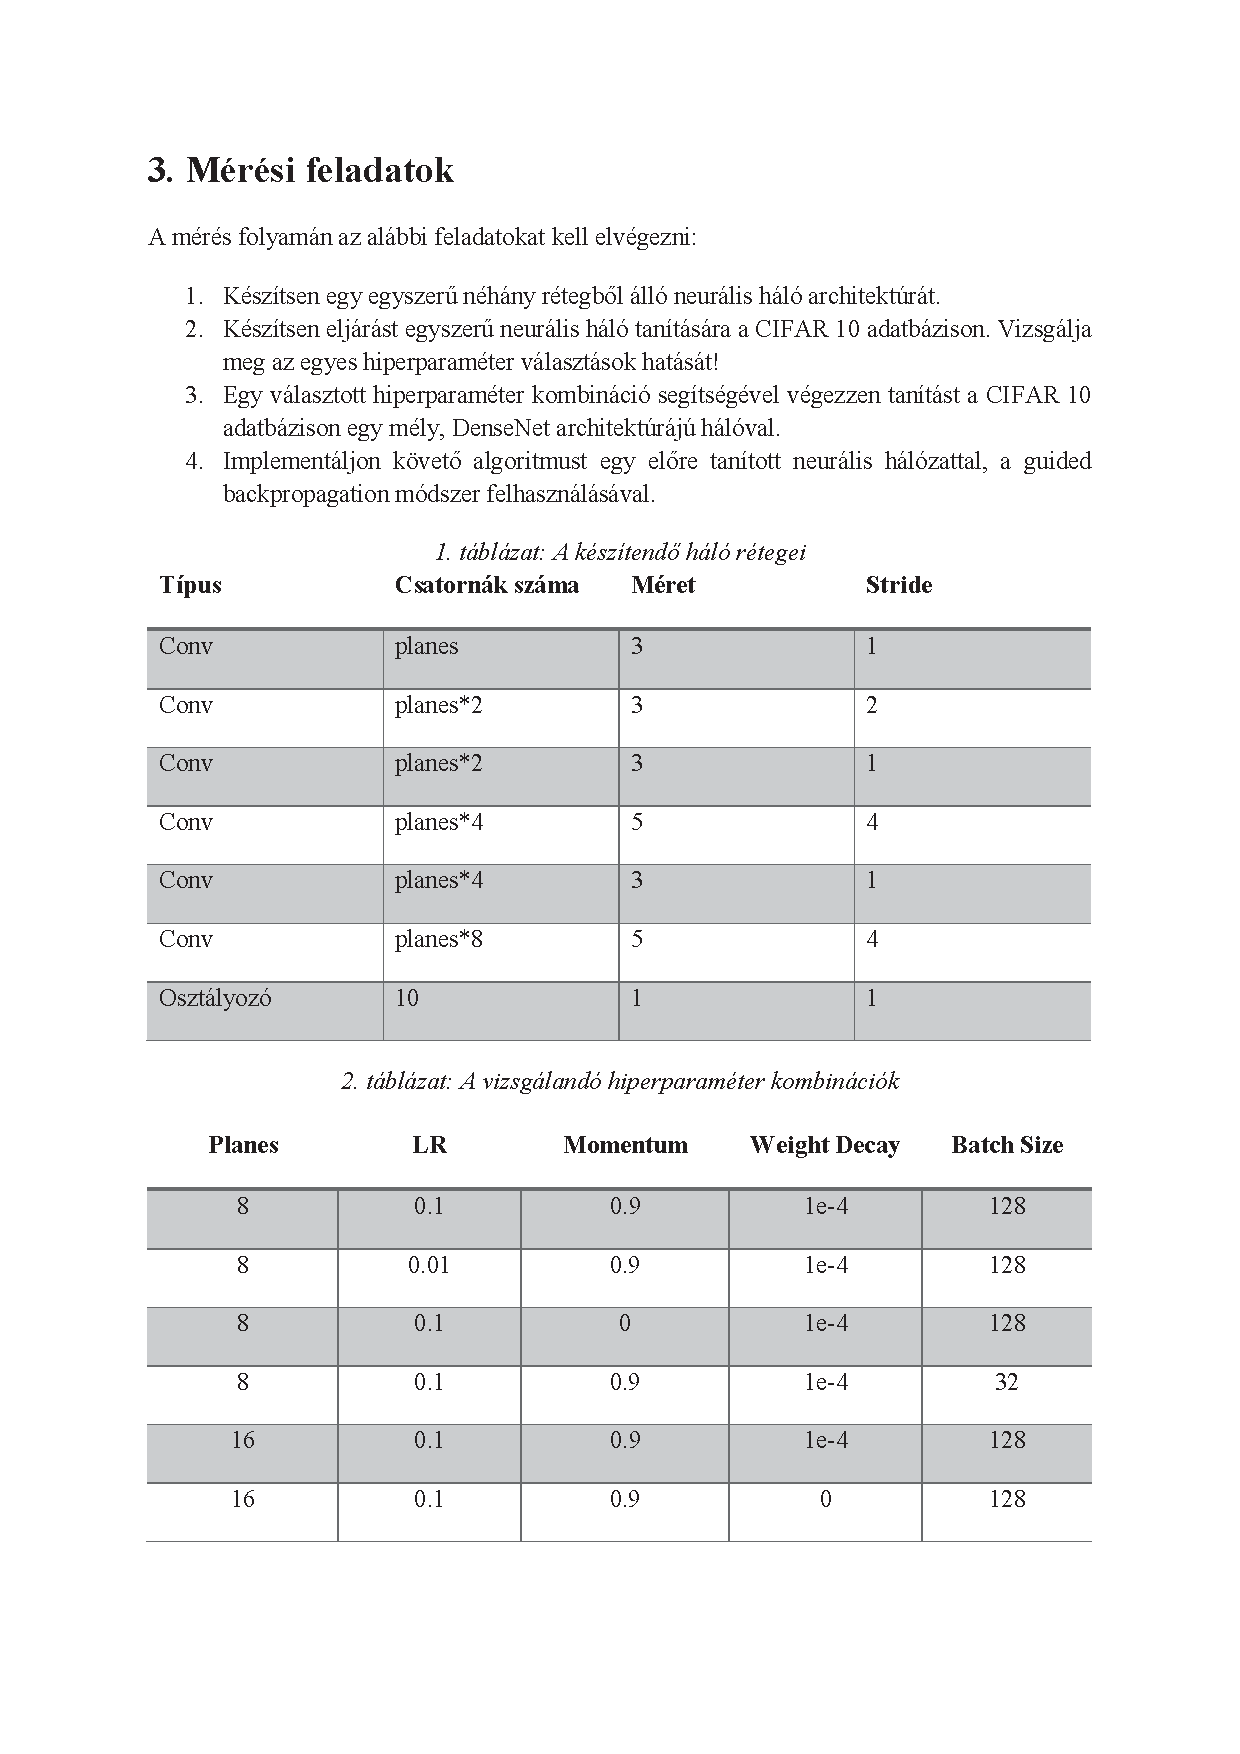
\includegraphics[trim = 25mm 210mm 20mm 33mm,clip, width=150mm,keepaspectratio]{figures/feladatok_m07.pdf}
%	\label{fig:Road-of-a-char}
%\end{figure}

A mérés folyamán az alábbi feladatokat kell elvégezni:
\begin{enumerate}
	\item \textbf{Valósítson meg egy egyszerű tempomatot!}
	
		Készítsen olyan Stateflow-modellt, amely képes a jármű sebességének irányítására a következő követelmények szerint. A \textit{SET} nyomógomb lenyomására a tempomat kapcsoljon be (a bekapcsolt állapotot a \textit{vehicle} blokk \textit{on/off} bemenetére továbbított 1-es értékkel is jelezze), és tartsa a gomb lenyomásakor érvényes sebesség-értéket. A tempomat a gázpedál lenyomására kapcsoljon ki! Az \textit{ON} nyomógomb hatására a tempomat szintén kapcsoljon be, és az előzőleg beállított sebességértékre gyorsítsa/lassítsa a járművet! Amennyiben még nincs beállított sebességérték, akkor az aktuális sebességet állítsa be. Biztonsági szempontból a tempomat 30 km/h sebesség alatt nem kapcsolható be.
		
		A megkívánt sebesség tartásához alkalmazzon P-szabályozót! Annak érdekében, hogy a jármű a beállított sebességet minél hamarabb elérje, ugyanakkor annak tartása ne hirtelen gázadással és gázelvétellel történjen, alkalmazzon más erősítésértéket az alapjel kis környezetében illetve azon kívül! Az erősítések értékét kísérleti úton állítsa be.
		
		A beavatkozó jel számítását a megfelelő állapotok \textit{during} műveleteiben érdemes elvégezni. Ne feledkezzen meg a diagram ébresztéséről!
	\item \textbf{Valósítson meg adaptív tempomatot!}
	
		Egészítse ki a működést a jármű előtti akadályok figyelésével is! A tempomatnak a gépkocsi előtt haladó járműtől biztonságos követési távolságot kell tartania. Ez a távolság sebességfüggő, mindig annyi, amekkora távolságot az adott sebességgel a jármű 3 másodperc alatt tesz meg. A követési távolság a beállított sebesség tartásánál fontosabb, így közeli akadály esetén olyan sebességet kell felvenni, amivel az akadály távolsága megfelel a biztonságos követési távolságnak. Az akadály megfelelő eltávolodása, illetve eltűnése esetén természetesen a jármű felgyorsítható a beállított sebességre.
		\newpage
	\item \textbf{Adjon ki figyelmeztetést balesetveszély esetén!}
	
		Amennyiben az akadály gyorsan közeledik (tehát a beért jármű sebessége jelentősen alacsonyabb az aktuális haladási sebességénél, esetleg éppenséggel áll), figyelmeztesse a vezetőt a veszélyre a \textit{warning} bemenetre \textbf{1} értéket továbbítva! A vészjelzés kikapcsolt tempomat mellett is legyen aktív.
\end{enumerate}
